\documentclass{article}

\usepackage{paper}
\usepackage{caption}

\setpapertitle{Models for Clustering with Arbitrary Shaped Clusters}

\setauthor{Sarthak Mittal}{150640}
\addauthor{Gurpreet Singh}{150259}
\addauthor{Debabrata Ghosh}{13817226}

\begin{document}
\makeheader

\abstract{
	Most real world data can be represented in simpler patterns in a possible lower dimensional manifold and the data can be generated through some non-linear mapping from this latent space to the observed space. We study a number of existing techniques that allow clustering of data by jointly representing the data in a lower dimensional latent form and performing clustering over this latent space. We present a generic generative story for such models and look at various number of ways to perform inference in different settings. We also present some discussion regarding mixture of experts and propose two models extending the latent clustering to form gate networks for better mixtures.
}

\begin{psection}{Introduction}

	Humans are capable of recognizing cluster patterns even when the shapes and sizes of the clusters are immensely varied. The intrinsic shortcoming of K-Means and Gaussian Mixture Models is that these models are able to properly cluster the data only when it can be represented in gaussian shaped clusters, and we need to specify the number of clusters. Though Dirichlet Process Mixture Models alleviate the latter problem of the model, it still tries to capture the data as a mixture of Gaussians.

	One of the most popular ways to solve this problem is by constructing a latent representation of the data and a complex non-linear function that can efficiently map the latent space representations to the data space representations. The latent representation can be thought of as a simple distribution like a mixture of Gaussians which is warped by a complex non-linear function to represent the data. Now, clustering on this latent representation by models that only allow gaussian-like cluster shapes still allow for arbitrary shaped clusters in the data space because of the non-linear warping functions.

	One way to approach the above problem is to first uncover a good latent representation of the data through some non-linear transformation techniques like a Gaussian Process variant of Probabilistic Principal Component Analysis \citep{gplvm} or using a Variational Autoencoder. Both of these constitute powerful non-linear function approximators and thus solve the problem well. Once we have the latent representation of the data, we perform clustering on the latent representation through some standard clustering techniques like Gaussian Mixture Model or Dirichlet Process Mixture Model. Thus, we get clusters of arbitrary shapes.

	The above technique, however, is not optimal because in doing so, we have made the task of latent representation and clustering mutually independent. Therefore, our model will be focused on finding a good latent representation which can be reconstruct our observations with high precision, but would not care about the inherent differences in the observations, \ie we would loose the inherent clustering present in the observations.

	However, we can see that these tasks are actually quite related to each other and any model would be able to construct more disambiguated latent representations if it performs the task of latent representation and clustering jointly. Thus, to efficiently solve the problem, we define a Generative Model where a vector in the latent space is sampled from a mixture of Gaussians (either a finite mixture or an infinite mixture) and then learn a complex non-linear function that maps the latent space to data space.

\end{psection}

\begin{psection}{Relevant Background}

	\begin{psubsection}{Variational Autoencoders}

		The key idea behind Variational Autoencoders \citep[VAEs,][]{VAE} is that any distribution in $D$ dimensions can be generated by taking a set of $D$ variables that are normally distributed and mapping them through a sufficiently complicated function \citep{vae-tut, VAE}. Hence, provided powerful function approximators, we can simply learn a function which maps independent, normally-distributed variables to the latent variables needed for our model, and these latent variables are then used to model the observations $\vX$, or rather the data distribution $\cD$ not known to us, from which the observations are assumed to be sampled.

		Therefore, the task is to find a strong non-linear mapping to approximate the latent variables needed to model the data distribution $\cD$. This mapping, in VAEs, is modelled using a neural network, and the mapping from these latent variables to the observations is through a distribution (generally exponential family) depending on the observed space $\cX$. For example, if $\cX = \bR$, then the estimated probability distribution for $\vx \sim \cD$ can be given as
		\begin{align*}
			\prob{\cD \pipe \vz} \qapprox \cP(\vX \pipe \vz; \vtheta) \eq \prod_{n} \ND{\vx_n \pipe f(\vz; \vtheta), \sigma^2 \vI}
		\end{align*}
		for some non-linear mapping $f: \brac{0, 1} \ra \bR$ (in this case) modelled using a neural network.

		The objective now is to compute the posterior over $\vz$ given the observations $\vX$. This would allow us to model the predictive posterior using samples of $\vz$ from this posterior. Since the posterior is intractable, we approximate the posterior $\prob{\vz \pipe \cD}$ using a proposal distribution $\cQ(\vz; \vphi)$. We use the standard VI strategy to estimate the posterior, by maximizing the ELBO bound, which is given as
		\begin{align*}
			\cL(\cQ) &\eq	- \kld{\cQ(\vz; \vphi)}{\prob{\vz \pipe \cD}} \\
			&\eq			\logp{\prob{\cD \pipe \vz}} - \kld{\cQ(\vz; \vphi)}{\prob{\vz}}
		\end{align*}

		This is similar to a Variational Inference (VI) objective. In fact, this is the VI procedure. However one problem with VI (with mean-field assumption) is that it models the parameters of each latent variable independently, and therefore we need an iterative procedure to model the proposal with respect to each variable. VAE tackles this problem by assuming that the latent variable is dependent on the input, and the mapping from the input to the parameters of the proposal distribution is modeled using a neural network. Since looking at the ELBO, one can say we wish to minimize the KL Divergence between the proposal and the prior for $\vz$ which is a standard Normal distribution, we can assume the proposal to be of the form $\ND{\vz \pipe \mu(\vx; \vphi), \sigma^2(\vx; \vphi)\,\vI}$. The negative ELBO is then considered as our loss, and the parameters (or weights) of the Neural Networks are learned using Backpropogation.

		This structure is similar to that of a standard autoencoder, where the network which maps the inputs to the parameters of the proposal is the encoder and the network mapping the sampled $\vz$'s to the parameters of the conditional likelihood distribution is the decoder.

		However, since we are assuming the variables $\vz$ to be sampled from the proposal, we cannot apply back propogation across the decoder and the encoder networks. This is handled using the reparameterization trick, $\vz = \eps \cdot \vsigma^2(\vx; \vphi) + \mu(\vx; \vphi)$. The working of a standard VAE is given in Figure \ref{fig:vae}.

		\begin{figure}[t]
			\centering
			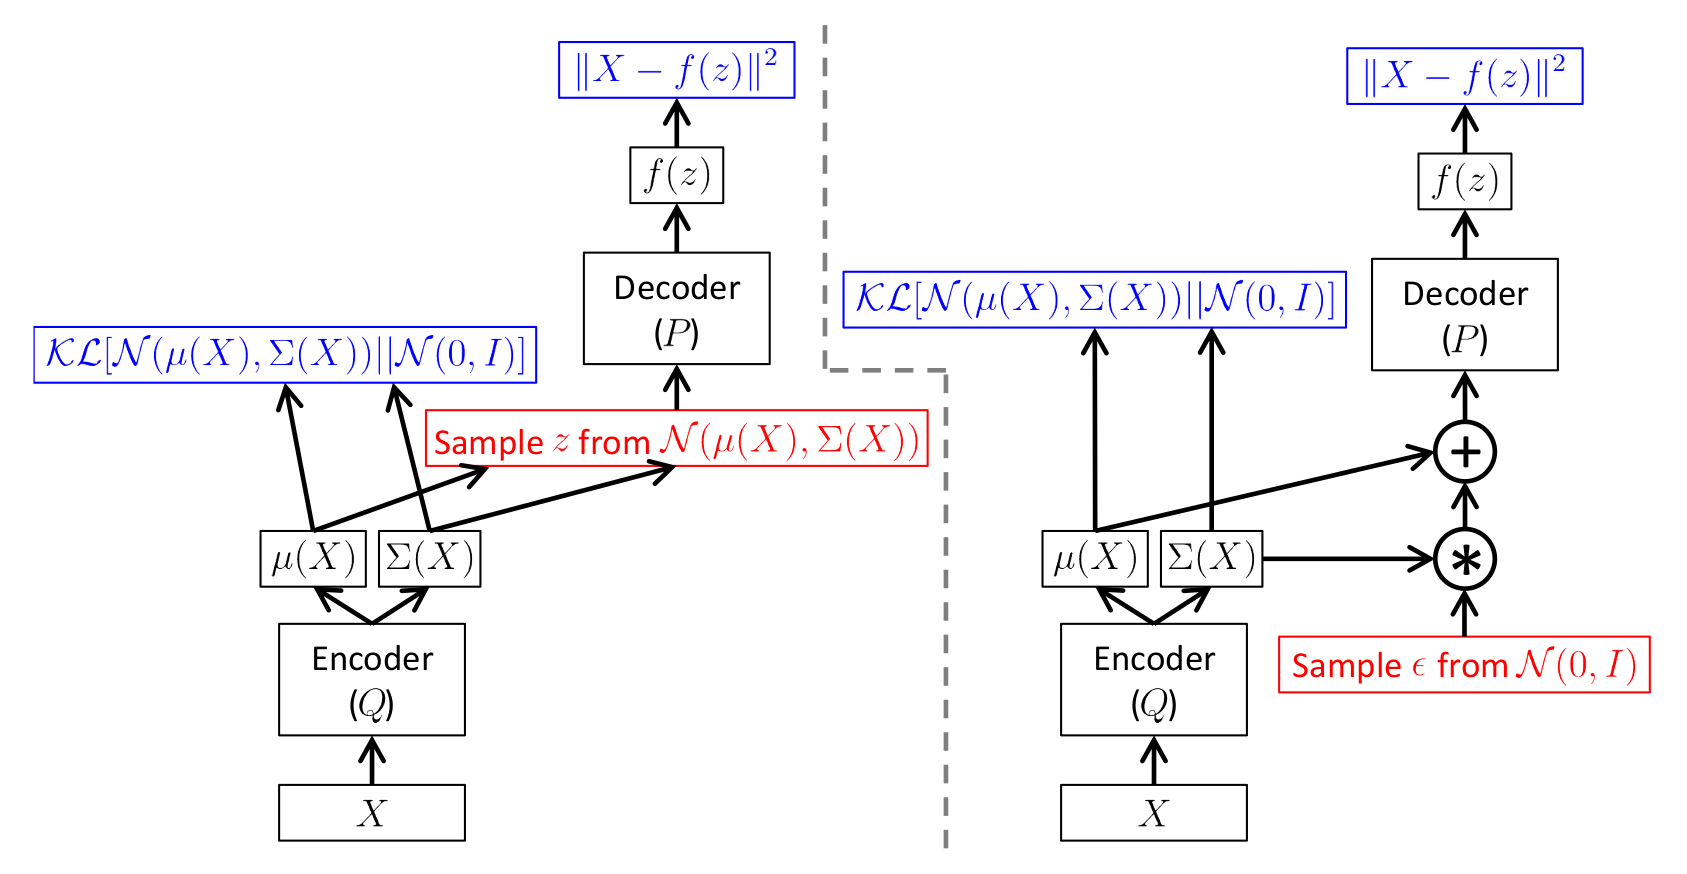
\includegraphics[width=0.8\textwidth]{includes/vae.png}
			\caption{Left: Without the reparameterization trick, Right: With the reparameterization trick}
			\label{fig:vae}
		\end{figure}

	\end{psubsection}

	\begin{psubsection}{Dirichlet Process Mixture Models}

		Similar to Dirichlet Processes or DPs are a family of stochastic processes.
		A Dirichlet process defines a distribution over probability measures $G : \Theta \ra \bR^+$, where, for any finite partition of $\Theta$, say $\set{\vtheta_k}_{k = 1}^K$, the random vector $\para{G(\vtheta_1), G(\vtheta_2) \dots G(\vtheta_K)}$ is jointly generalized under a Dirichlet Distribution \citep{murphy} \footnote{G(\vtheta) is a random variable since $G$ itself is a random measure and is sampled from the Dirichlet Process}, written as
		\begin{align*}
			\para{G(\vtheta_i), G(\vtheta_2) \dots G(\vtheta_K)}	\qsim	\tfunc{Dir}{\alpha G_0(\vtheta_1), \alpha G_0(\vtheta_2) \dots \alpha G_0(\vtheta_K)}
		\end{align*}
		where $\alpha$ is called the concentration parameter and $G_0$ is the base distribution. $\alpha G_0$ collectively is called the base measure.

		Dirichlet processes are really useful in the task of non-parametric clustering, using a mixture of Dirichlet Processes \citep{dp-ferg, dp-anto} (commonly DP Mixture Models or Infinite Mixture Models).
		In fact, a DP Mixture Model can be seen as an extension of Gaussian Mixture Models over a non-parametric setting.

		The basic DP Mixture Model follows the following generative story
		\begin{align*}
			\mdef{Likelihood}			\vy_n \pipe \vtheta_n	&\qsim	F(\vy_n \pipe \vtheta_n) &\\
			\mdef{Conditional Prior}	\vtheta_n \pipe G			&\qsim	G \\
			\mdef{Hyperparameter}				G						&\qsim	\tfunc{DP}{G_0, \alpha}
		\end{align*}
		where $G \sim$ DP denotes sampling from a Dirichlet Process given a base measure.

		When we are dealing with DP Mixture Models for clustering, it helps to integrate out $G$ with respect to the prior on $G$. \citep{neal}. Therefore, we can write the clustering problem in an alternate representation, although the underlying model remains the same.
		\begin{align*}
			\mdef{Likelihood}			\vy_n \pipe c_n, \Phi	&\qsim	F(\vy_n \pipe \vphi_{c_n}) & \\
			\mdef{Latent Distribution}	c_n \pipe \vp			&\qsim	\tfunc{Discrete}{p_1, p_2 \dots p_K} \\
			\mdef{Priors}				\vphi_k					&\qsim	G_0 & \\
			&&							\vp						&\qsim	\tfunc{Dir}{p_1, p_2 \dots p_K}
		\end{align*}
		where $c_n$ is the cluster assignment for the $n$\tth point and $\Phi = \set{\vphi_k}_{k = 1}^{K}$ are the likelihood parameters for each cluster. $K$ denotes the number of clusters, and being a non-parametric model, we assume $K \ra \infty$.

		If the likelihood and the base distribution are conjugate, we can easily derive a posterior representation for the cluster assignments or the latent classes, and use inference techniques such as Mean Field VB \citep{blei} and Monte Carlo Markov Chain \citep{esc-west, neal}.	\et{Neal} also describes various inference methods in case of non-conjugate base distribution.

		Dirichlet processes are extremely useful for clustering purposes as they do not assume an inherent base distribution, and therefore it is possible to apply Dirichlet Process priors over complex models.

	\end{psubsection}

	\begin{psubsection}{Stick-Breaking VAE}
		Stick-Breaking Variational Autoencoder ~\citep{nalisnick2016deep} is a recent model that aims to combine the Variational Autoencoder structure with Bayesian Nonparametrics. Fairly novel and ingenious, it combines Stick-Breaking process with the Variational Autoencoder structure by making the latent representations of data-points an infinite dimensional probability vector. This latent representation is accomplished by having a stick-breaking process that generates the latent representation $\vpi$, given as
		\begin{align*}
			\pi_{n,1} &\eq \beta_1 \\
			\pi_{n,l} &\eq \beta_l \prod_{l' = 1}^{l - 1} (1 - \beta_{l'}) \\
			&\text{and so on...} \\
			\beta_{i} &\sim \text{Beta}(1,\alpha)
		\end{align*}
		This makes the latent representation unbounded and hence we get a nonparametric model combined with the Variational Encoder. There are a couple of problems that need to be addressed before the model can work. The problems are related mainly to inference since the latent dimension has unbounded dimension, performing inference would be a highly non-trivial task. Moreover, there is also the problem that we cannot use Beta distribution to model the posterior in the inference as we know that Beta distribution is not a location-scale distribution and thus cannot be reparameterized into a distribution independent of the parameters (unlike a Gaussian Distribution). More precisely, a Beta distribution cannot be represented in the form of a Differentiable, Non-centered parameterization.

		We first look at the general problem of inference. To tackle the infinite dimensionality problem, the paper proposes to use an inference procedure similar to Variational Inference for Dirichlet Process Mixture Models, proposed by \cite{blei2006variational}. To accomplish this, there is a truncation level enforced on the variational distribution. Note that this truncation of the variational posterior distribution does not imply a finite dimensional latent representation since the truncation level is a parameter of the variational distribution and not the model specification. Hence the latent representation of the model still has unbounded dimensions.

		Having solved the problem of general inference in the model, we look at the problem of back-propagating through the Beta distribution, that is making this distribution free of the parameters emitted by the neural network so that variance is controlled in training and backpropagating does not involve a non-differentiable layer that will prohibit gradient descent. This is achieved by using approximate distributions in place of the standard Beta distribution. The paper uses the Kumaraswamy Distribution, which is defined as follows:
		\begin{align*}
			\tfunc{Kumaraswamy}{x \pipe a, b} &\eq a\,b\,x^{a - 1} \para{1 - x^a}^{b - 1} \qquad x\in(0,1)\quad a,b>0
		\end{align*}
		The paper mentions that for $a=1$ or $b=1$ or both, the Kumaraswamy and Beta distributions are equivalent and for equivalent parameter settings, the Kumaraswamy Distribution resembles the Beta distribution but has a higher entropy. Moreover, Kumaraswamy Distribution can be written in a differentiable, non-centered parameterization as
		\begin{align*}
			x &\sim (1-u^{1/b})^{1/a} \\
			u &\sim \text{Uniform}(0,1)
		\end{align*}
		Hence, sampling from this distribution is easy and also its KL-divergence with a Beta distribution can be obtained in closed form. We further note that the paper also mentions a Gaussian-Probit Parameterization with a logistic function as another possibility.

		Having dealt with all the necessities, this model can now be trained using Stochastic Gradient Variational Bayes ~\citep{VAE}, just like a standard Variational Autoencoder is trained but with the above modifications. There is one more small caveat though, the KL-Divergence term of the Kumaraswamy-Beta distribution reveals a Digamma function and an infinite taylor series sum. During implementation, the infinite taylor series sum needs to be approximated properly using required number of terms and the Digamma function's derivative, the polygamma function, is difficult to implement and hence the digamma function is further approximated using a taylor series expansion.
	\end{psubsection}

\end{psection}

\begin{psection}{Survey of Models for Clustering with Arbitrary Shaped Clusters}

	The task at hand is to model the latent variables such that there is inherent clustering with the latent variables, and which can effectively generate samples from the real distribution $\cD$, represented by a set of observations $\vX$. We first present a generic generative story for such models, and then look at various implementations of the generative story.

	Since we want the latent variables to be clustered, we can assume a Finite or Infinite Gaussian Mixture Prior over the latent variables, where the infinite case is handled using Dirichlet Process. Therefore, we assume that the mixture weights are sampled either from a Dirichlet Distribution or a Stick-Breaking Process. We represent a generalized prior, say MM which could mean either a Dirichlet or Stick-Breaking Distribution.

	Since we are assuming a mixture of gaussians for the prior, a natural prior on the parameters of each gaussian is a Normal Inverse-Wishart Prior. The last step is to sample $\vx$, which is done through a non-linear mapping from the latent variables to the parameters of the distribution of $\vx$ which we represent by $\cP$ and will depend on the domain that $\vx \sim \cD$ belongs to.

	Using these steps, the complete generative story is given in \hyperlink{algo:1}{1}.

	\begin{algo}[0.8\textwidth]{Generative Story for a Clustering Model}

		\begin{enumerate}
			\item Draw mixture weights $\vpi \sim \tfunc{MM}{\alpha}$
			\item For each component $k = 1 \dots K$
				\begin{enumerate}
					\item Draw gaussian parameters $\vmu_k, \vSigma_k \sim \tfunc{NIW}{\vlambda}$
				\end{enumerate}
			\item Draw model parameters $\vtheta \sim \prob{\vtheta}$
			\item For each observation $n = 1 \dots N$
				\begin{enumerate}
					\item Draw latent cluster assignment $c_n \sim \tfunc{Multinoulli}{\vpi}$
					\item Draw latent coordinates $\vz_n \sim \ND{\vmu_{c_n}, \vSigma_{c_n}}$
					\item Draw sample $\vx_n \sim \cP(\vx \pipe f(\vz_n; \vtheta), \vgamma)$
				\end{enumerate}
		\end{enumerate}

		The given generative story is a plausible generative model for any data as it only assumes that even though data exists in a complex manifold there exists a disentangled simpler representation of the data that explains it well, which is often true, even for real-world data. The question now boils down to constructing expressive variational distributions and performing efficient inference such that the data is most expressively represented in a latent space.

	\end{algo}

	We first take a look at a model which allows us to have a non-parametric (Infinite Gaussian Mixture) prior on the latent variables, however suffers from slow inference and no notion of reconstruction.

	\begin{psubsection}{Infinite Warped Mixture Model}

		Following the generic story (Algorithm \hyperlink{algo:1}), the Infinite Warped Mixture Model \cite[IWMM, ][]{iwmm} assumes that the observations are sampled has coordinates in a latent space and was generated through some non-linear functional mapping from the latent space to the data space.

		To tackle the problem of manifold clustering for arbitrary shaped clusters, the infinite Warped Mixture Model (iWMM) \citep{gplvm} assumes that the latent coordinates are generated from a Dirichlet Process Mixture Model and these coordinates are mapped to the observations in data space through some complex non-linear function which is modeled using a Gaussian Process.

		As mentioned earlier, we use the stick-breaking process to generate mixture weights for a Dirichlet process with parameter $\valpha$. Also, since the non-linear mapping is defined by a function sampled from a Gaussian Process, we need to modify the generative story where instead of sampling $\vtheta$, we directly sample $f$ from a gaussian process with a defined mean and a kernel function.

		Since the model uses Gaussian Process and Dirichlet Process to jointly learn latent representations and arbitrary shaped clusters, the inference scheme in the procedure is non exact and non trivial. Inference in accomplished through a Sampling based approximate inference scheme, the general structure of which is:

		\begin{enumerate}
			\item For each observation n $= 1,...,N$, sample the cluster assignment $z_n$ by Collapsed Gibbs Sampling
			\item Sample latent coordinates $X$ and kernel parameters using Hybrid Monte Carlo
		\end{enumerate}

		Thus, by constructing a latent manifold on which the data exists and learning a complex non-linear function, the model is able to both accurately uncover clusters and estimate density of the data even when the shapes of the clusters are very varied and non-Gaussian like. The disadvantage of this problem, though, is that since the model uses Gaussian process and Sampling scheme for inference, the complexity of the model increases with the amount of data we have, and thus inference is performed with the comlpexity of each iteration being $\mathcal{O}(N^3)$. Thus, though the model is very powerful, it doesn't scale well and is slow to train.

		The next models we discuss aim to solve this problem using VAEs, which allow for faster inference without losing on model complexity.

	\end{psubsection}

	\begin{psubsection}{InfoGAN}
		InfoGAN \citep{chen2016infogan} is an information-theoretic extension to Generative Adversarial Network (GAN) \citep{goodfellow2014generative}, which is a type of implicit-density generative model. A vanilla GAN works by having two networks, a generator network $G$ and a discriminator network $D$ and the model optimization is modelled by a game between the generator and the discriminator. To be more precise, $G$ maps some latent distribution like $\mathcal{N}(0,I)$ to the data distribution and $D$ has the task of discriminating between the true data distribution and the data distribution to which $G$ maps the latent distribution.

		This is achieved by sampling from the latent distribution and the true data distribution and then using $G$ to get the generated distribution and $D$ to discriminate between the two. The optimization works in the way that $G$ has to generate samples that can fool $D$ while $D$ has to learn to discriminate between the generated points and true points. This sort of game-theoretic objective has an equilibrium governed by the principle of Nash Equilibrium. Thus, $D$ and $G$ play the two-player minimax game with the value function:
		\begin{align*}
			\min_G \max_D V(G, D) \eq \E[\vx \sim p_{\text{data}}]{\logp{D(\vx)} + \E[\vz \sim p_z]{\log{1 - D(G(\vz))}}}
		\end{align*}

		Though this vanilla version of GAN is able to generate very realistic looking samples, it cannot be used to cluster the data. However, the information theoretic extension InfoGAN improves upon the vanilla GAN by using a latent code $\vz$ that can be decomposed into an uncompressible noise and a latent code $\vc$ which targets the salient structured semantic features of the data distribution. The InfoGAN works by maximizing the mutual information between the generated data and the latent code $\vc$. This information theoretic regularization maintains high mutual information between the latent code $\vc$ and the generator distribution. That is, $I(\vc;G(\vz,\vc))$ should be high. Note that $I(\;\cdot\;)$ is the difference of the two entropy terms:
		\begin{align*}
			I(X;Y) = H(X) - H(X|Y) = H(Y) - H(Y|X)
		\end{align*}

		This modifies the objective value function, and the new value function could be seen to be the following:
		\begin{align*}
			\text{V}_{new}(G,D) = \text{V}(G,D) - \lambda I(\vc;G(\vz,\vc))
		\end{align*}

		Denote the true posterior as $P(\vc|\vx)$ and the approximating auxiliary distribution as $Q(\vc|\vx)$. Since calculating the mutual information $I(\vc;G(\vz,\vc))$ requires access to the posterior distribution, the paper aims to maximize a lower bound of the mutual information, which has been obtained to be the following:
		\begin{align*}
			I(\vc;G(\vz,\vc)) &\qge \E[\vx\sim G(\vz,\vc)]{\E[\vc' \sim P(\vc|\vx)]{log\, Q(\vc'|\vx)}} + H(\vc) \\
			&\eq					L_1(G, Q)
		\end{align*}

		Note that $L_1(G,Q)$ can be maximized w.r.t $Q$ directly and w.r.t. $G$ via the reparameterization trick. Hence, the final InfoGAN is defined as a minimax game with a variational regularization of the mutual information with the hyperparameter $\lambda$ as:
		\begin{align*}
			\min_{G,Q} \max_D \ V_{\text{InfoGAN}}(G,D,Q) \eq V(D,G) - \lambda L_1(G,Q)
		\end{align*}

		With this objective, by using a latent code that follows a Categorical (Multinoulli) distribution, we can obtain an implicit clustering on the data as well as a good generative model.
	\end{psubsection}

	\begin{psubsection}{Structured Variational Autoencoder}
		Though the iWMM model is very efficient at uncovering the number of clusters and the cluster shapes, it does not scale well to large amounts of data. To solve this issue, GMM-SVAE \citep{svae} defines the required non-linear functional mapping through a neural network, which have been proved to be universal function approximators. The model takes advantage of the fact that Variational Autoencoders work well in problems of density estimation and hence, on combining VAEs with GMM, the model is able to uncover arbitrary shaped clusters.

		This model follows the exact generative story presented in Algorithm \hyperlink{algo:1}{1}. The prior on the latent variables is given by a finite mixture model, and therefore the MM prior defines a Dirichlet prior for SVAE

		The model performs inference by using recognition networks to produce local evidence potentials which are then incorporated in the general graphical model inference algorithm that sits on top. It uses a conditional random field (CRF) variational family and learns recognition networks that output conjugate graphical model potentials instead of complete variational distribution's parameters. These potentials are then used in the graphical model inference algorithms in place of non-conjugate likelihoods.

		\begin{pssubsection}{Inference}

			The inference scheme used in the model is fairly complex but we try to give the formal structure of the inference. We use different notation from the original paper so that the notation is consistent throughout the report.

			We define a general conjugate exponential family model having global parameters $\vgamma$ and local latent variables $\vz = \set{\vz_n}_{n = 1}^N$. We define $\prob{\vz \pipe \vgamma}$ as exponential family and $\prob{\vgamma}$ as its conjugate prior. Hence, we have
			\begin{align*}
				\prob{\vgamma}			&\eq	\texp{\dotp{\eta_{\vgamma}^0}{t_\vgamma(\vgamma)} - \logp{\func{Z_\vgamma}{\eta_{\vgamma}^0}}} \\
				\prob{x \pipe \vgamma}	&\eq	\texp{\dotp{\eta_z^0(\vgamma)}{t_z(\vz)} - \logp{\func{Z_z}{\eta_x^0(\vgamma)}}} \\
				&\eq \texp{\dotp{t_\vgamma(\vgamma)}{\brac{t_z(\vz), 1}}}
			\end{align*}
			where the last equality is written by leveraging exponential family conjugacy structure. Now we model $\func{\cP}{\vx \pipe \vz, \vtheta}$ by a general distribution (e.g. Neural Network) and have the exponential family prior $\prob{\vtheta}$ on $\vtheta$.

			Now for inference, we consider a general mean field assumption with variational distribution $\cQ(\vgamma) \cQ(\gamma) \cQ(x)$. The variational inference objective reduces to maximizing the following ELBO:
			\begin{align*}
				\cL \brac{\cQ(\vgamma) \cQ(\vtheta) \cQ(x)} &\eq \E[\cQ(\vgamma) \cQ(\vtheta) \cQ(x)]{\log{\frac{\prob{\vgamma} \prob{\vz \pipe \vgamma} \prob{\vx \pipe \vz,\vtheta}}{\cQ(\vgamma) \cQ(\vtheta) \cQ(x)}}}
			\end{align*}
			Now, we take $\cQ(\vgamma)$ to be in the same exponential family as the prior $\prob{\vgamma}$ and we denote its natural parameters by $\eta_\vgamma$. We restrict $\cQ(\vtheta)$ to be in the same exponential family as $\prob{\vtheta}$ with natural parameters $\eta_\vtheta$. We restrict $\cQ(x)$ to be in the same exponential family as $\prob{\vz \pipe \vgamma}$ with natural parameters $\eta_z$.

			Having done this, we now present the novelty in the inference scheme followed by the authors. They chose the variational parameter $\eta_x$ as a function of the parameters $\eta_\vgamma$ and $\eta_\vtheta$. They claim that a natural choice is to have $\eta_x$ as the local partial optimizer of $\mathcal{L}$. However due to lack of conjugacy structure, finding the local optimizer would be computationally expensive. Hence instead, $\eta_x$ is chosen as the local partial optimizer of a surrogate objective $\hat{\mathcal{L}}$ which has conjugacy structure, given by:
			\begin{align*}
				\hat{\mathcal{L}}(\eta_\vgamma, \eta_z, \vphi) &= \E[\cQ(\vgamma) \cQ(\vz)]{\logp{\frac{\prob{\vgamma} \prob{\vz \pipe \vgamma} \texp{\psi(\vz; \vx, \vphi)}}{\cQ(\vgamma) \cQ(\vz)}}} \\
				\psi(\vz; \vx, \vphi) &\eq \dotp{r(\vz; \vphi)}{t_z(\vz)}
			\end{align*}
			where $\{r(\vz; \vphi)\}$ is a parameterized class of functions obtained using a recognition model. Note that the potentials $\psi(\vz; vx,\phi)$ have a conjugate form to $\prob{\vz \pipe \vgamma}$. Hence, we obtain the variational distribution $\vQ(\vz)$ and the variational parameter $\eta_z$ as:
			\begin{align*}
				\eta_z^{*}(\eta_\vgamma,\phi) &\eq \argmax{\eta_z} \hat{\mathcal{L}}(\eta_\vgamma, \eta_z, \vphi) \\
				\cQ^{*}(\vz) &\eq \texp{\dotp{\eta_z^{*}(\eta_\vgamma,\phi)}{t_z(\vz)} - \logp{Z_z(\eta_z^{*}(\eta_\vgamma, \vphi))}}
			\end{align*}

			Having obtained the local optimum value of $\eta_z$, we can update the other variational parameters $\eta_\vgamma$ and $\eta_\vtheta$ using gradients of the following expression of $\cL_{\text{SVAE}}$ (we have to maximize it):
			\begin{align*}
				\cL_{\text{SVAE}} &\eq	\E[\cQ(\vgamma) \cQ(\vtheta) \cQ^{*}(\vz)]{\logp{\frac{\prob{\vgamma} \prob{\vz \pipe \vgamma} \prob{\vx \pipe \vz, \vtheta}}{\cQ(\vgamma) \cQ(\vtheta) \cQ^{*}(\vz)}}} \\
				&\eq 					\E[\cQ(\vtheta) \cQ^{*}(\vz)]{\logp{\cP(\vx \pipe \vz, \vtheta)}} - \kld{\cQ(\vgamma) \cQ^{*}(\vz)}{\prob{\vgamma, \vz}} - \kld{\cQ(\vtheta)}{\prob{\vtheta}}
			\end{align*}
			This can be obtained using Reparameterization trick and automatic differentiation. Note that we can obtain natural gradients in this case.

			The disadvantage of the model is that it has been worked on only in the parametric setting where the number of clusters present in the data is provided to the network. Hence, though the model efficiently learns the shapes of the clusters, it doesn't give us the number of clusters present in the data. At the same time, it is worth pointing out that this model, through the use of Neural Networks, scales up to increasing amounts of data very efficiently.

		\end{pssubsection}

	\end{psubsection}

	\begin{psubsection}{Structured Inference Network}
		Structured Inference Network (SIN) ~\citep{lin2018variational} is a very recent work that aims to combine Probabilistic Graphical Models (PGMs) with Deep Neural Networks (DNNs). It builds up on the work of Structured Variational Autoencoders and extends it by simplifying and generalizing the methodology of SVAE ~\citep{svae}. The main idea behind this model is that it incorporates the graphical model structure in the inference network of variational autoencoders, thereby giving us both the flexibility of Neural Networks along with an interpretable and powerful graphical model sitting behind it. 

		Assuming we have data $\vx_1,...,\vx_N$ and we are modelling the data using latent variables $\vz_1,...,\vz_N$ that have a probabilistic graphical model over them. Thus, the SIN uses the following joint distribution:
		\begin{align*}
			p(\vx,\vz,\theta) &= \underbrace{[\prod_{n=1}^N p(\vx_n|\vz_n,\vtheta_{NN})]}_\text{DNN}\; \underbrace{\vphantom{\prod_{n=1}^N}[p(\vz|\vtheta_{PGM})]}_\text{PGM}\; \underbrace{\vphantom{\prod_{n=1}^N}[p(\vtheta_{PGM})]}_\text{Hyperprior}
		\end{align*}
		We know that Structured Variational Autoencoders aim to solve similar problems using mean-field variational inference and a two-stage iterative procedure. The advantage is that if the variational family over $\vz$ is chosen conjugate with the PGM structure sitting on $\vz$, inference can be performed. However, the inference is equivalent to an implicitly constrained optimization which is difficult to solve. Moreover, this inference procedure does not work if the prior contains non-conjugate terms. SIN can, however, preserve some structure even if the graphical model contains non-conjugate factors.

		Structured Inference Networks work by having a variational distribution with a certain structure. From below, we assume $\vtheta$ to be deterministic, that is, it does not have any prior. This proposed structure consists of two types of factors, and can be written as:
		\begin{align*}
			q(\vz|\vx,\vphi) &= \frac{1}{\mathcal{Z}(\vphi)} \underbrace{[\prod_{n=1}^N q(\vz_n|\vf_{\phi_{NN}}(\vx_n))]}_\text{DNN Factor}\; \underbrace{\vphantom{\prod_{n=1}^N}[q(\vz|\vphi_{PGM})]}_\text{PGM Factor}
		\end{align*}
		Note that the role of the DNN term is to enable flexibility while the role of the PGM term is to incorporate model structure. To perform efficient inference, there are certain conditions that need to be met. Firstly, the normalizing constant $\mathcal{Z}(\vphi)$ is easy to evaluate and differentiate. Secondly, we can draw samples from the distribution, that is $\vz^{*}(\vphi) \sim q(\vz|\vx,\vphi)$. Moreover, an additional desirable though not required feature is the ability to compute the gradient of $\vz^{*}(\vphi)$ using the reparameterization trick.

		Now, if these conditions are met, a stochastic gradient of the lower bound can be obtained in a way similar to VAEs ~\citep{VAE}. The variational lower bound can be written as follows:
		\begin{align*}
			\mathcal{L}(\vtheta,\vphi) &= \mathbb{E}_q[log\, \frac{p(\vx,\vz|\vtheta)}{q(\vz|\vx,\vphi)}] \\
			&= \underbrace{\sum_{n=1}^N \mathbb{E}_q[log\,\frac{p(\vx_n|\vz_n,\vtheta_{NN})}{p(\vz_n|\vf_{\phi_{NN}}(\vx_n))}]}_\text{Similar to VAE} + \underbrace{\vphantom{\sum_{n=1}^N}\mathbb{E}_q[log\,p(\vz|\vtheta_{PGM})]}_\text{Due to Structured Prior} - \underbrace{\vphantom{\sum_{n=1}^N}\mathbb{E}_q[log\,q(\vz|\vphi_{PGM})] + log\,\mathcal{Z}(\vphi)}_\text{Due to PGM term in inference}
		\end{align*}
		Now, for our problem, the PGM required is a Gaussian Mixture Model. Hence, the model's PGM structure and the variational distribution can be defined as follows for efficient inference:
		\begin{align*}
			p(\vz|\vtheta_{PGM}) &= \prod_{n=1}^N [\sum_{k=1}^K \mathcal{N}(\vz_n|\vmu_k,\vSigma_k)\pi_k] \\
			q(\vz|\vx,\vphi) &= \frac{1}{\mathcal{Z}(\vphi)}\prod_{n=1}^N \underbrace{\vphantom{\sum_{k=1}^K}[\mathcal{N}(\vz_n|\vm_n,\vV_n)]}_\text{DNN Factor}\;\underbrace{[\sum_{k=1}^K \mathcal{N}(\vz_n|\Bar{\vmu}_k,\Bar{\vSigma}_k)\Bar{\pi}_k]}_\text{GMM Factor}
		\end{align*}
		Having this setting of the model satisfies the conditions required for the Structured Inference Network and thus structured, amortized, efficient inference can be performed on the model. Thus we see that SIN is a very powerful and recent approach that combines PGM structure with Neural Networks very efficiently.
	\end{psubsection}

	\begin{psubsection}{Variational Deep Embedding}
		Variational Deep Embedding (VaDE) was proposed by \cite{vade}. It is a simplistic model than the previous models discussed, and greatly simplifies the generic generative story by assuming a uniform prior on the cluster means, variances, and misture proportions. Also, it assumes a uniform prior on the model parameters $\vtheta$.

		\begin{figure}[h]
			\centering
			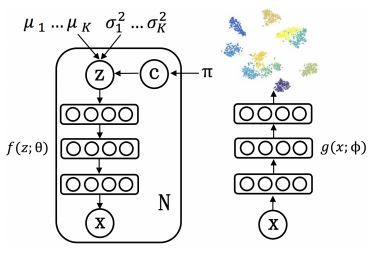
\includegraphics[height=150px]{includes/vade.jpg}
			\caption{(Left) Plate Notation for VaDE and (Right) an encoder network $g(\vx; \phi)$}
			\label{fig:my_label}
		\end{figure}

		Assuming whether the observations $\vx$ is binary or real-valued we compute $\mu_x = f(\vz, \vtheta)$ and choose a sample $\vx \sim Ber(\mu_x)$ or compute $[\mu_x;\log\sigma^2_x] = f(\vz,\vtheta)$ and choose a sample $\vx \sim \mathcal{N}(\mu_x,\sigma^2_x\vI)$. From the generative story, the joint probability can be written as
		\begin{align*}
			\prob{\vx, \vz, c} \eq \prob{\vx \pipe \vz, \vtheta} \prob{\vz \pipe c} \prob{c}
		\end{align*}

		An instance of VaDE is tuned to maximize the likelihood of the given data points. Given the generative process described above we have
		\begin{align*}
			\logp{\prob{\vx}} &\eq \log{\int_\vz \sum_c \prob{\vx, \vz, c} \id \vz} \\
			&\qge \E[\cQ(\vz, c \spipe x)]{\logp{\frac{\prob{\vx, \vz, c}}{\cQ(\vz, c \pipe \vx)}}} \eq \cL_{\text{ELBO}}
		\end{align*}
		where $\cQ(\vz, c \pipe \vx)$ is the proposal distribution.

		Mean field is assumed on the proposal distribution, giving:
		\begin{align*}
			\cQ(\vz, c \pipe \vx) &\eq \cQ(\vz \pipe \vx) \cQ(c \pipe \vx)
		\end{align*}

		Similar to VAE, the distribution $\cQ(\vz \pipe \vx)$ is modelled using a neural network $g$ as follows
		\begin{align*}
			\tilde{\vmu}, \logp{\tilde{\vsigma}^2} &\eq g(\vx, \vphi) \\
			\cQ(\vz \pipe \vx) &\eq \ND{\vz \pipe \tilde{\vmu}, \tilde{\vsigma}^2 \vI}.
		\end{align*}

		Further, a decoder model is added giving the following:
		\begin{align*}
			\prob{\vx \pipe \vz} &\eq \prob{\vx \pipe f(\vz, \vtheta)}
		\end{align*}

		The authors use an interesting approach to ``approximating'' the proposal distribution $\cQ(c \pipe \vx)$, which although looks absurd, in practice works surprisingly well. First, one can realize, the ELBO can be re-written in the following manner,
		\begin{align*}
			\cL_{\text{ELBO}} &\eq 	\E[\cQ(\vz, c \spipe \vx)]{\logp{\frac{\prob{\vx, \vz, c}}{\cQ(\vz, c \pipe \vx)}}} \\
			&\eq					\int_{\vz} \sum_{c} \cQ(c \pipe \vx) \cQ(\vz \pipe \vx) \set{\logp{\frac{\prob{\vx \pipe \vz} \prob{\vz}}{\cQ(\vz \pipe \vx)}} + \logp{\frac{\prob{c \pipe \vz}}{\cQ(c \pipe \vx)}}} \\
			&\eq \int_{\vz} \cQ(\vz \pipe \vx) \logp{\frac{\prob{\vx \pipe \vz} \prob{\vz}}{\cQ(\vz \pipe \vx)}} \id \vz - \int_{\vz} \cQ(\vz \pipe \vx) \kld{\cQ(c \pipe \vx)}{\prob{c \pipe \vz}} \id \vz
		\end{align*}

		In order to maximize the above ELBO, it seems we need to minimize the aberage KL Divergence over the latent variables, when sampled using the posterior. \et{Jiang et al.} approximated this simply using only one sample of $\vz$ and therefore, we can write 
		\begin{align*}
			\cQ(c \pipe \vx) \eq \prob{c \pipe \vz = \hat{\vz}} \eq \frac{\prob{c} \prob{\vz = \hat{\vz} \pipe c}}{\sum_{c' = 1}^{K} \prob{c'} \prob{\vz = \hat{\vz} \pipe c'}}
		\end{align*}
		where $\hat{\vz}$ is a sample from the posterior proposal $\cQ(\vz \pipe \vx)$.

		Given the simplicity of the model, we performed some experiments on it. We implemented the complete model on Tensorflow from scratch, and performed experiments on a couple of datasets. This is discussed in detail in the following section.
	\end{psubsection}

	\begin{psubsection}{Experiments on Clustering with VaDE}

		\begin{pssubsection}{MNIST Dataset}

			We firstly performed a set of experiments on the MNIST Dataset, which is a collection of hand-written digits providing 55000 training examples and 5000 test examples, with each digit an image of dimensions 28x28. We further binarized the images with a threshold of 0.5.

			We performed unsupervised clustering on the model using VaDE, and compared the results with a plugin clustering model, where a latent representation is learned using a VAE and a GMM is learned over the latent variables for the observations.

			We first describe the training process and then show the results of our experiments. Since we want to maximize the ELBO defined previously, our loss is simply the negative of the ELBO. Also, since we are working with binary data, the likelihood is given by a multivariate bernoulli.

			Further, the expectation with respect to the latent variables is approximated using Monte Carlo estimation with a single sample point, generated from the approximate posterior of the latent variables, $\cQ(\vz \pipe \vx)$. Therefore, we can write the final term for the ELBO as

			\begin{figure}[h!]
				\centering
				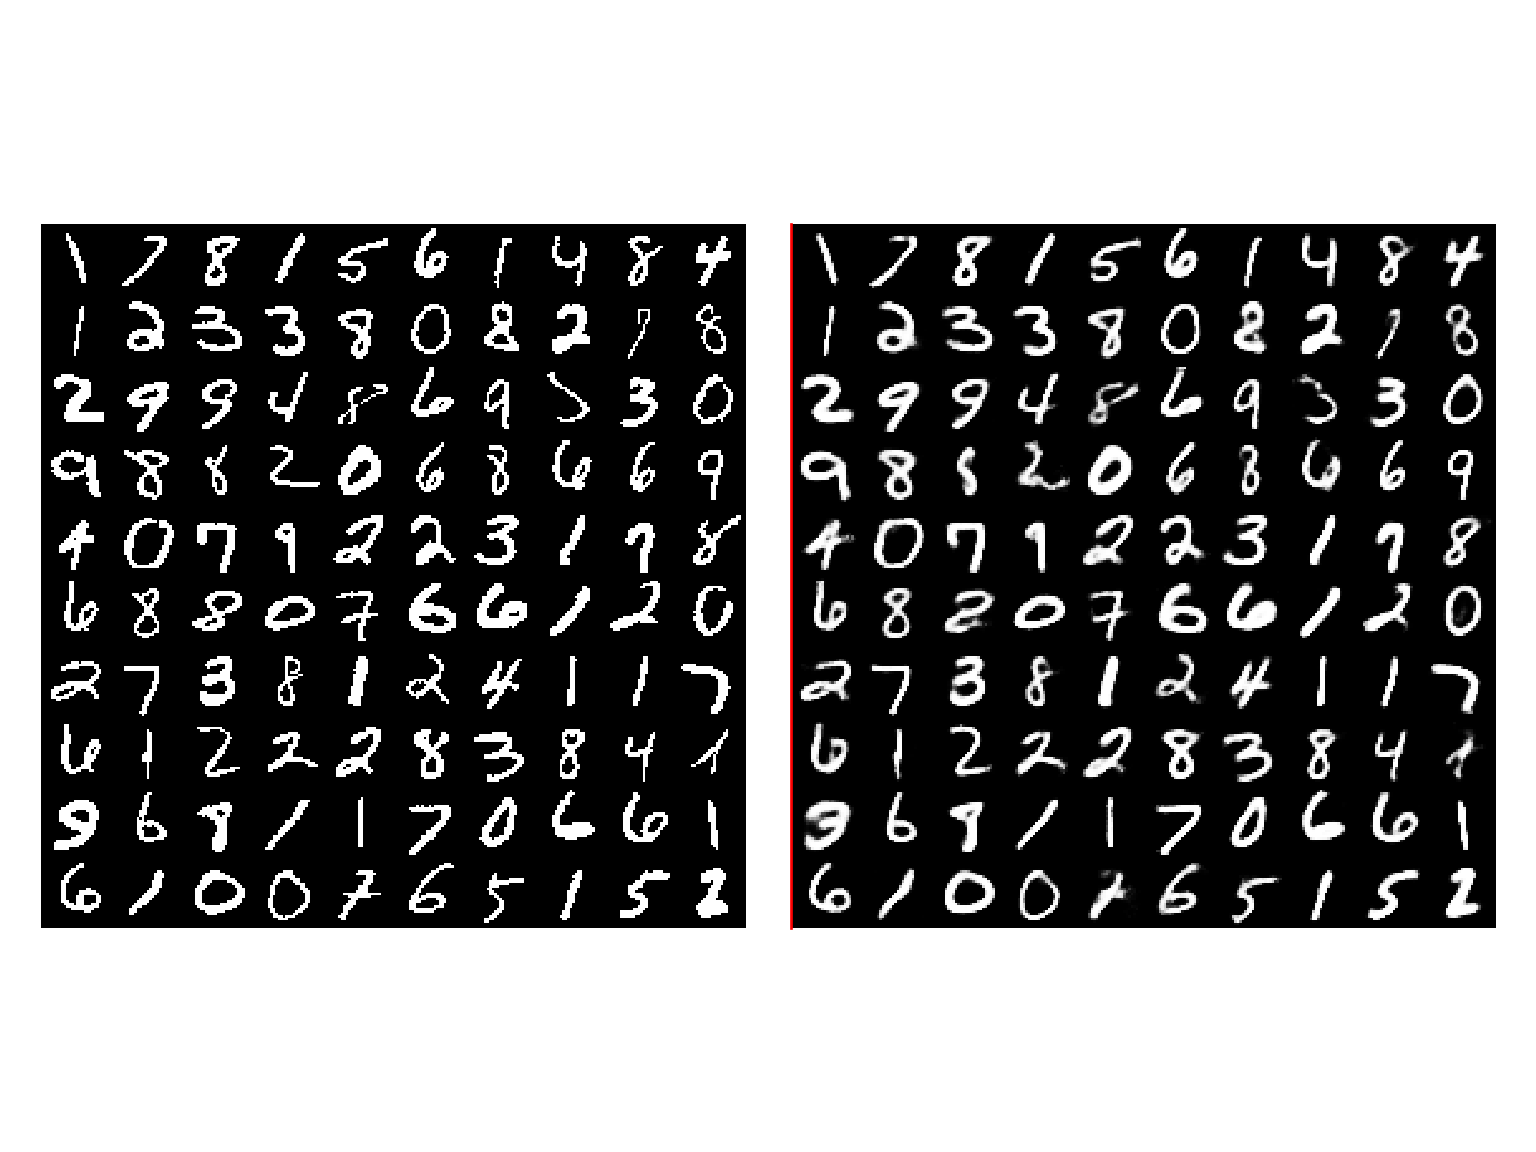
\includegraphics[width=0.8\textwidth, trim={0.5 2.1cm 0.5 2.1cm}, clip]{includes/plots/mnist/recon-initial.png}
				\caption{Plug-in Clustering -- Left: Original digits, Right: Reconstructed Digits}
				\label{fig:gmm-recon}
			\end{figure}

			\begin{figure}[h!]
				\centering
				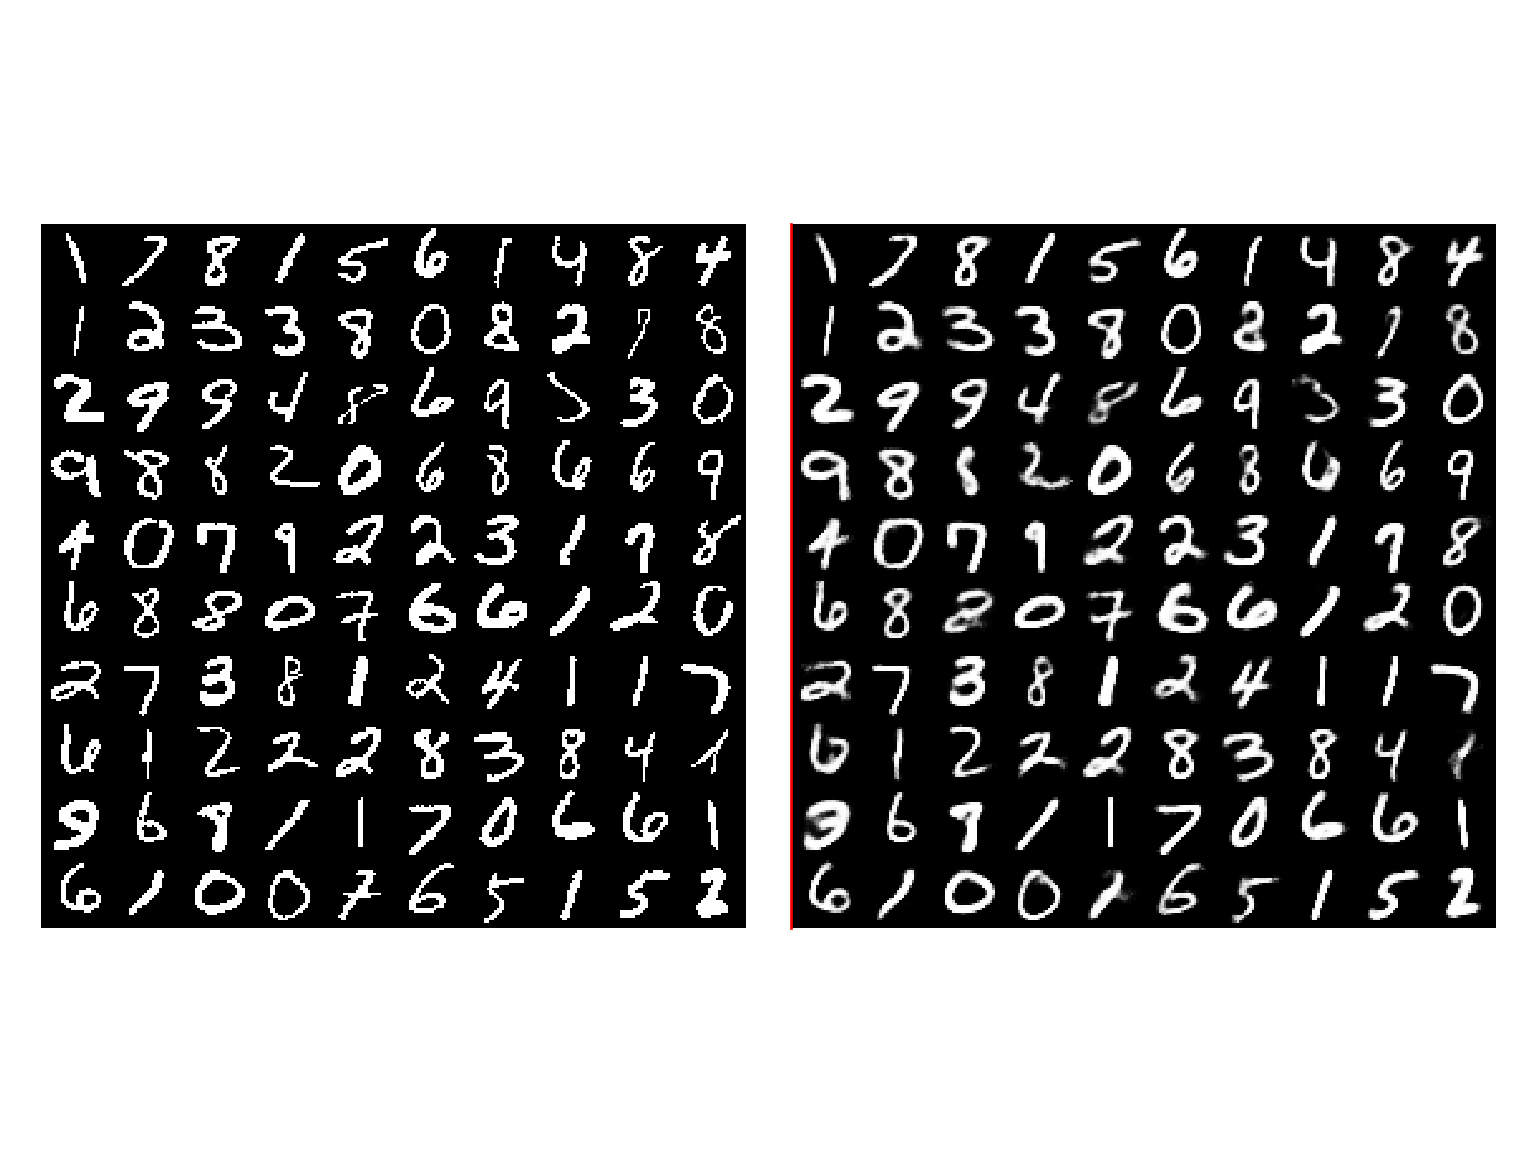
\includegraphics[width=0.8\textwidth, trim={0.5 2.1cm 0.5 2.1cm}, clip]{includes/plots/mnist/recon-final.png}
				\caption{VaDE Clustering -- Left: Original digits, Right: Reconstructed Digits}
				\label{fig:vade-recon}
			\end{figure}

			\begin{align*}
				\cL_\text{ELBO} &\eq \frac{1}{N} \sum_{n = 1}^N \sum_{d = 1}^D \set{\vx_d \log{\vmu_x^{(n)}|_d} \sum_{d = 1}^D \para{1 - \vx_d} \log{1 - {\vmu_x^{(n)}}|_d}} \\
				&\hspace{1.1em} -\quad \frac{1}{2} \sum_{c = 1}^K \gamma_c \sum_{j = 1}^J \set{\logp{\vsigma_c^2|_j} + \frac{{\tilde{\vsigma}^2}|_j}{\vsigma_c^2|_j} + \frac{\para{\tilde{\vmu}|_j - {\vmu_c}|_j}^2}{{\vsigma_c^2}|_j}} \\
				&\hspace{1.1em} +\quad \sum_{c = 1}^K \gamma_c \logp{\frac{\pi_c}{\gamma_c}} + \frac{1}{2} \sum_{j = 1}^J \para{1 + \logp{{\tilde{\vsigma}^2}|_j}}
			\end{align*}

			\begin{figure}[h!]
				\centering
				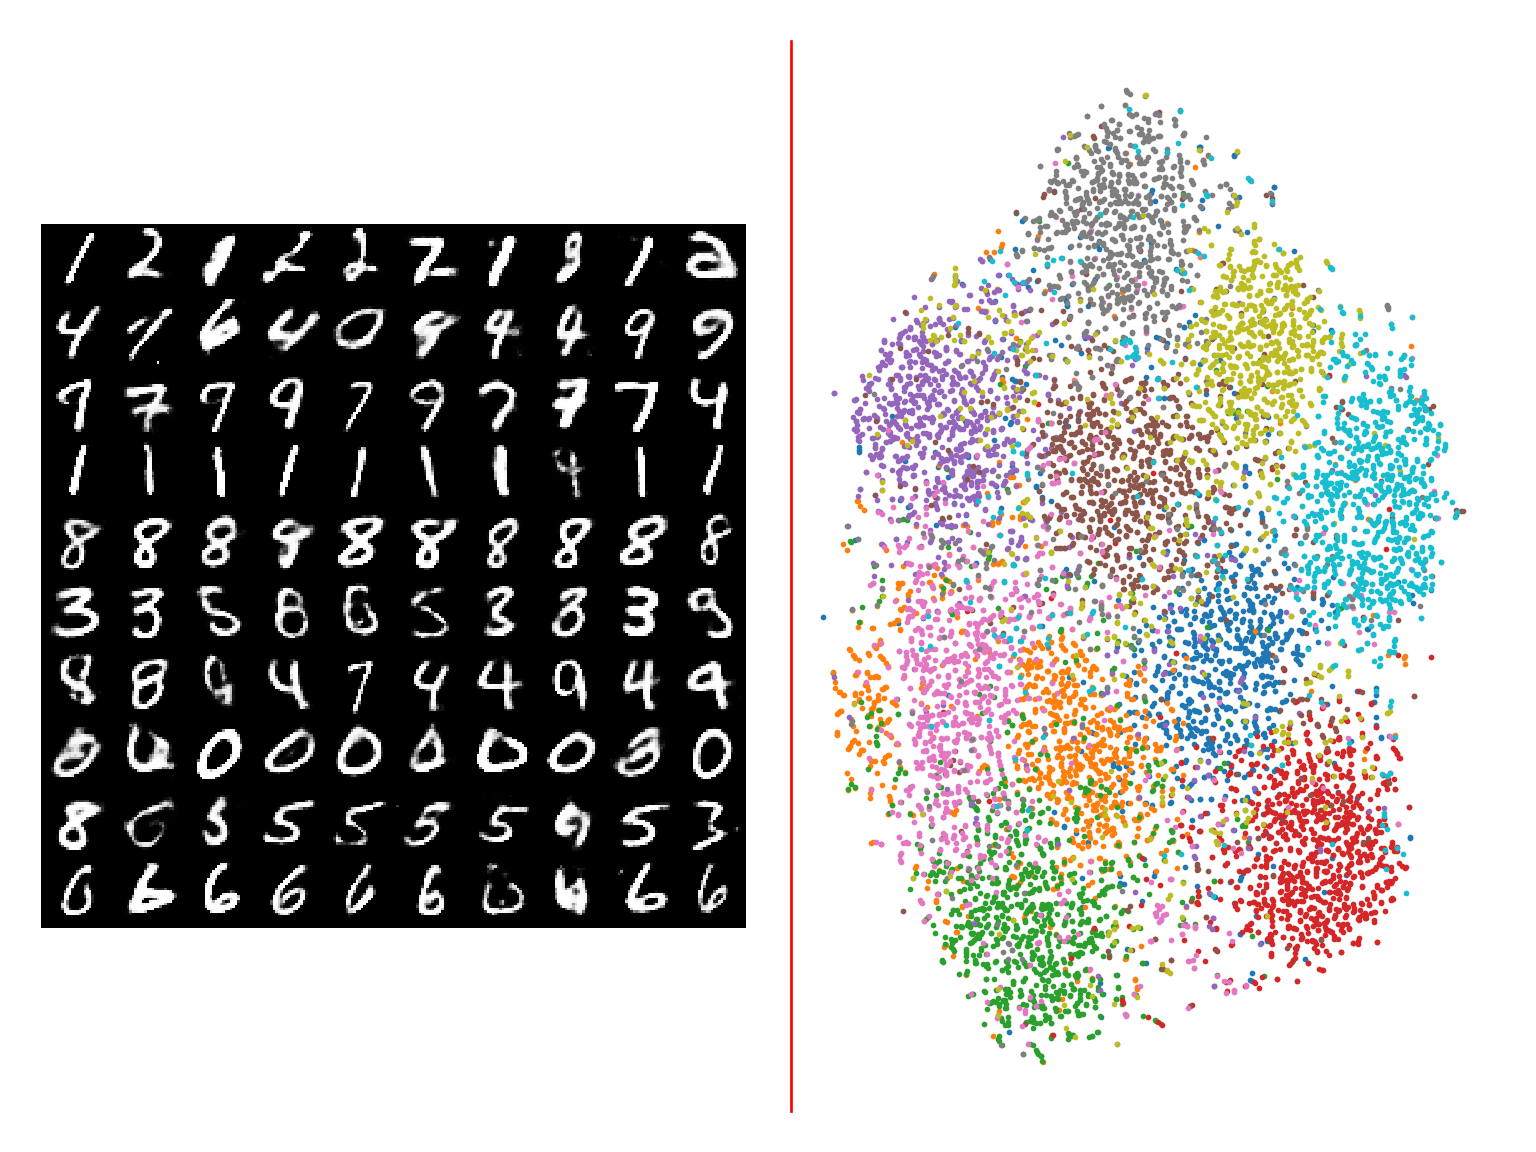
\includegraphics[width=0.8\textwidth, trim={0.5 0.8cm 0.5 0.8cm}, clip]{includes/plots/mnist/sample-initial.png}
				\caption{Plug-in Clustering -- Left: Sampled Digits with row representing cluster, Right: TSNE Plot}
				\label{fig:gmm-sample}
			\end{figure}

			\begin{figure}[h!]
				\centering
				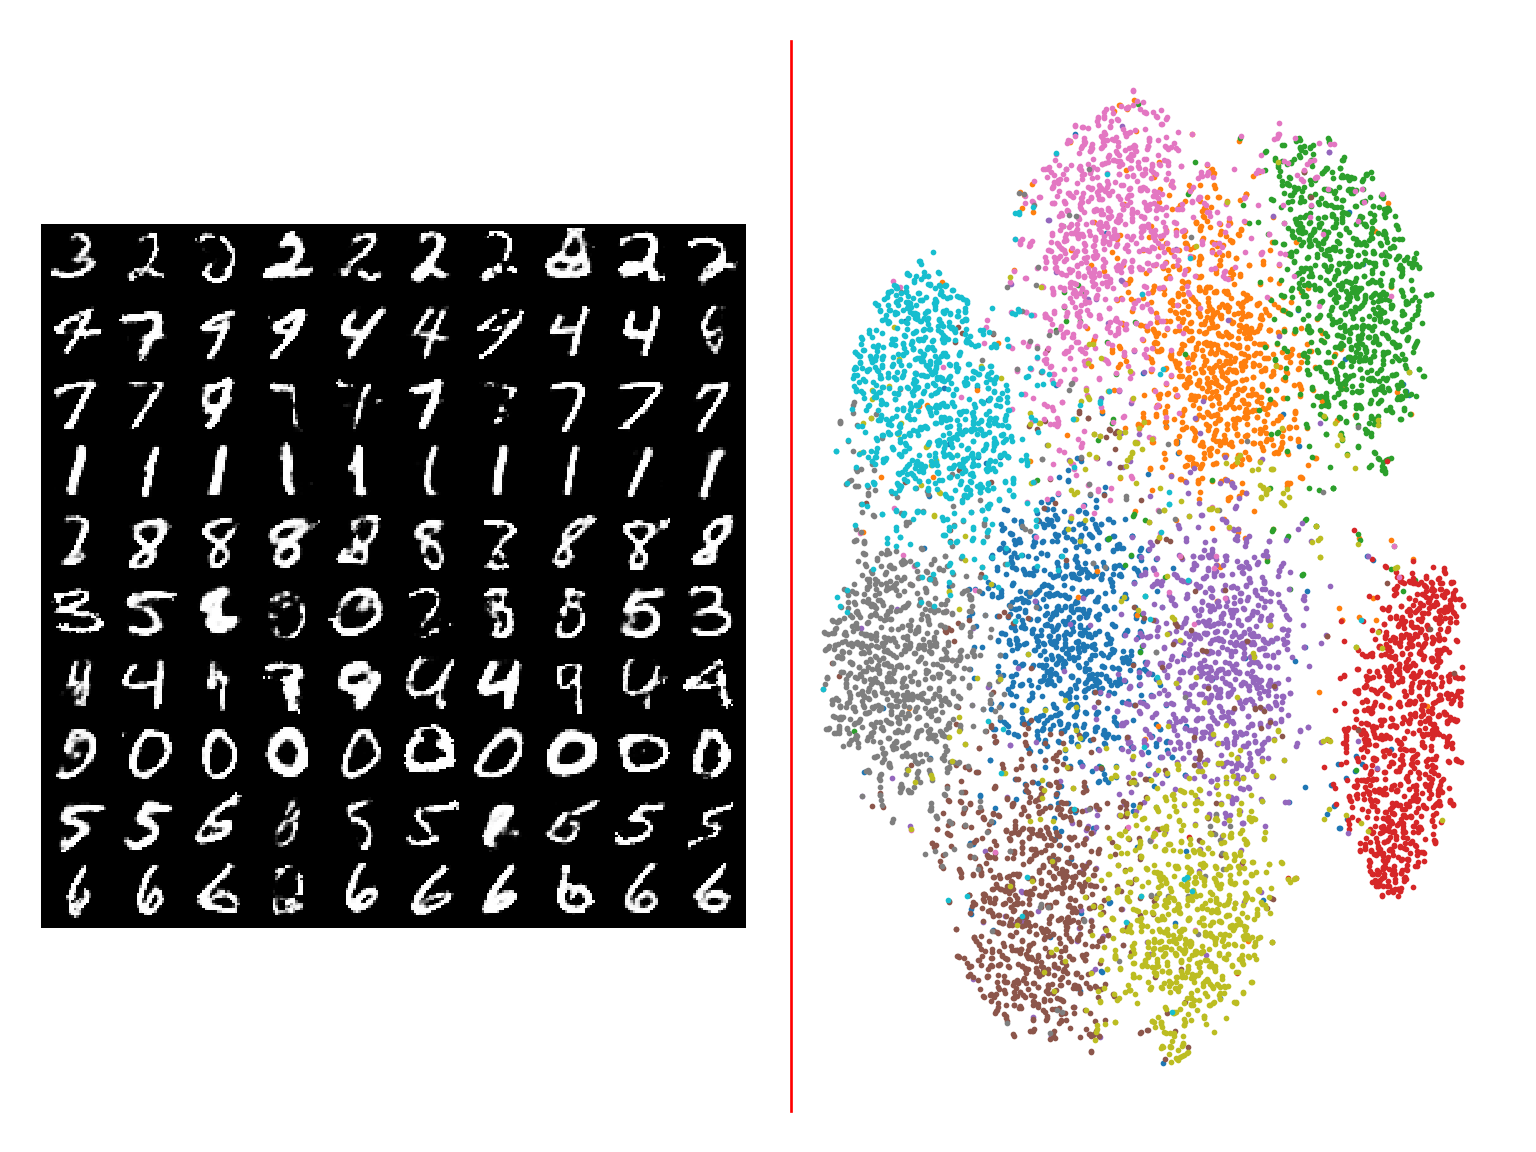
\includegraphics[width=0.8\textwidth, trim={0.5 0.8cm 0.5 0.8cm}, clip]{includes/plots/mnist/sample-final.png}
				\caption{VaDE Clustering -- Left: Sampled Digits with row representing cluster, Right: TSNE Plot}
				\label{fig:vade-sample}
			\end{figure}

			The loss / negative ELBO is minimized using an Adam optimizer. There was another interesting observation made by the authors, which we as well found in our experiments, that using Adam optimizer works on even the GMM parameters, including the mixture proportions, inspite of the fact that we are performing unconstrained optimization, when the GMM mixture components are clearly constrained.

			We first compare the reconstruction of the VAE for the plug-in case and the VaDE Case. The reconstruction plots are given in Figures \ref{fig:gmm-recon} and \ref{fig:vade-recon} respectively for plug-in and VaDE case. One can see that the the reconstruction in case of VaDE is slighly lesser, however there is minimal difference and therefore conclude that inspite of adding a different prior to the latent variables, the reconstruction power of the VAE is not lost.

			We further compare the effeciency of the clustering algorithms, which can be seen in Figures \ref{fig:gmm-sample} and \ref{fig:vade-sample} respectively for plug-in and VaDE models. It is clear that there is much lesser ambuigity in clustering when using VaDE model, and also the TSNE plot clearly shows there are larger gaps between clusters, and therefore, we can conclude VaDE outperforms the direct plug-in clustering model.
			
			\begin{remark}
				The lower quality digits in the sampled plot are due to no thresholding on the predictive posterior, and would be greatly improved if some thresholding is added. Also, the lower quality in case of VaDE is more profound here, however proper thresholding and longer training runs would get rid of such loss. We show, in Figure \ref{fig:thresholded-sampling}, samples generated by controlling the variance while sampling.
				
				We thus see that by controlling the predictive variance, we get very good results where the clusters are representative of different digits. We note that the model still struggles with some disambiguations (e.g. between 4 and 9). Moreover, the model is quite sensitive to initializaiton as some runs lead to perfect disambiguations between the classes while some runs result in a particular class split into two different clusters while some classes are merged into one cluster.
			\end{remark}
			
			\begin{figure}
			    \centering
			    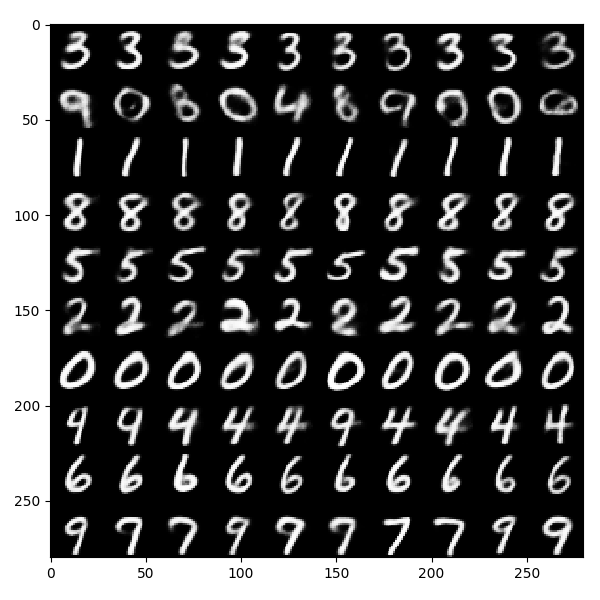
\includegraphics[width=0.4\textwidth]{includes/plots/mnist/sample-thresh-initial.png}
			    \hspace{0.5cm}
			    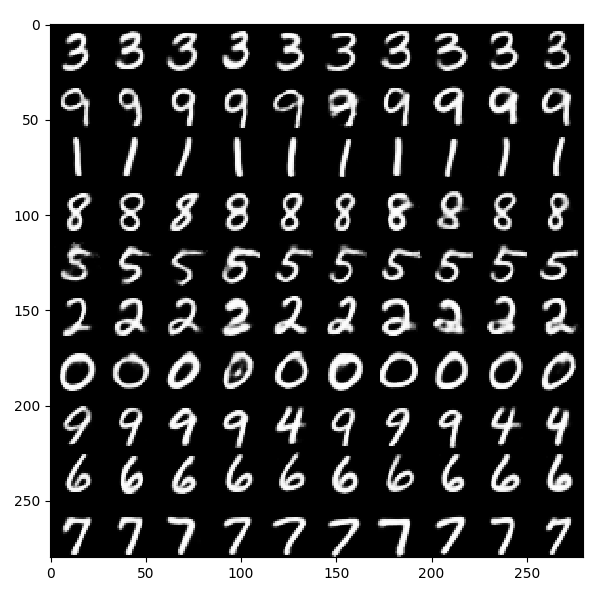
\includegraphics[width=0.4\textwidth]{includes/plots/mnist/sample-thresh-final.png}
			    \caption{Left: Samples with Thresholding for plug-in model and Right: Samples with Thresholding for VaDE model}
			    \label{fig:thresholded-sampling}
			\end{figure}

			We further look at the usability of VaDE for clustering where the observations are real valued.
		\end{pssubsection}

		\begin{pssubsection}{Spiral Dataset}

			This is a toy dataset on which we run the VaDE model in order to analyze the performance of VaDE. Since the observations are real valued in this case, we can rewrite the loss, exactly as done in previous case, but with a gaussian likelihood, and for simplicity's sake, with a known variance.

			\begin{figure}[h!]
				\centering
				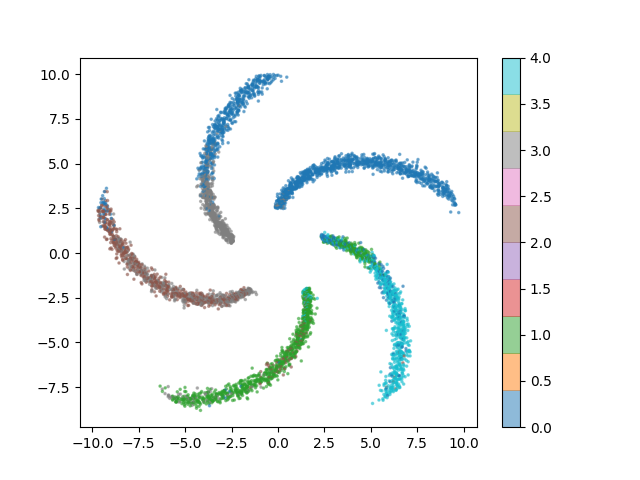
\includegraphics[width=0.4\textwidth, trim={2.8cm 1.8cm 5.65cm 2cm}, clip]{includes/plots/spiral/clustered-gmm.png}
				\hspace{0.5cm}
				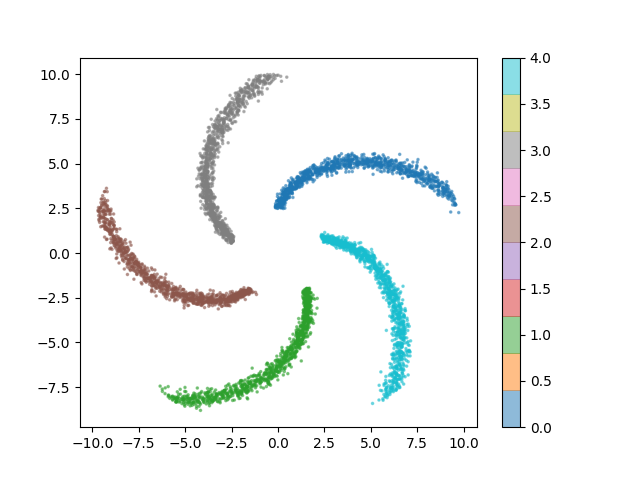
\includegraphics[width=0.4\textwidth, trim={2.8cm 1.8cm 5.65cm 2cm}, clip]{includes/plots/spiral/clustered-vade.png}
				\caption{Left: Clustering with plug-in model, Right: Clustering with VaDE model}
				\label{fig:spiral-cluster}
			\end{figure}

			In Figure \ref{fig:spiral-cluster}, we have shown the training data after clustering, both using plug-in model (left) and VaDE model (right). It can be seen that there is better clustering in the case of VaDE model where the clusters seem to be pure, which is not the case with plug-in model. The superiority of VaDE in this case is even more clear when one looks at the TSNE plots in Figure \ref{fig:spiral-tsne}.

			\begin{figure}[h!]
				\centering
				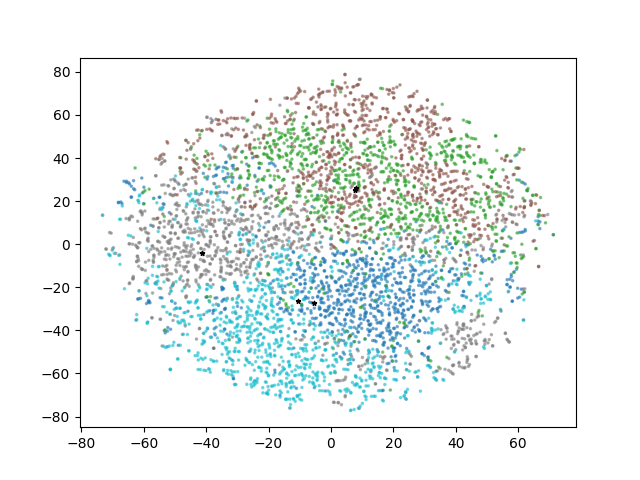
\includegraphics[width=0.4\textwidth, trim={2.8cm 1.8cm 2.1cm 2cm}, clip]{includes/plots/spiral/tsne-gmm.png}
				\hspace{0.5cm}
				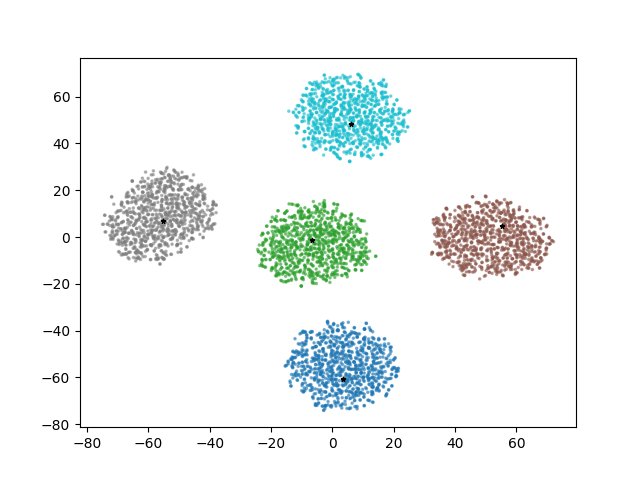
\includegraphics[width=0.4\textwidth, trim={2.8cm 1.8cm 2.1cm 2cm}, clip]{includes/plots/spiral/tsne-vade.png}
				\caption{Left: TSNE of clusters with plug-in model, Right: TSNE of clusters with VaDE model}
				\label{fig:spiral-tsne}
			\end{figure}
		\end{pssubsection}
	\end{psubsection}

	With this, we conclude the models we surveyed for our report. In the next section, we present a model we propose, combining the power of VAEs and non-parametric models, and apply this for the purpose of clustering, same as above.
\end{psection}

\begin{psection}{Relevant Extensions}
	\begin{psubsection}{DPMM-SVAE}
		Our aim is to come up with a model that not only recovers the complex shaped clusters in the data, but also the number of clusters present. Moreover, it should scale well to large amounts of data. To solve this problem, we propose a model similar to the GMM-SVAE model described above. However, instead of having a finite mixture model at the prior like the GMM-SVAE model, we propose to have a Dirichlet Process Mixture Model sitting at the top. This allows creating of new clusters as more and more data is seen.

		To achieve this aim, we describe the generative story as given in \hyperref{algo:2}{2}

		\begin{algo}[0.8\textwidth]{Generative Story for DPMM-SVAE}

			\begin{enumerate}
				\item Draw mixture weights $\vpi \sim Gem(\valpha)$
				\item {For each component $k = 1 \dots \infty$
						\begin{enumerate}
							\item Draw $(\vmu_k, \vSigma_k) \sim NIW(\vlambda)$
					\end{enumerate}}
				\item Draw parameters of the encoder and decoder model $\vtheta \sim \prob{\vtheta}$kd
				\item For each obsevation n $= 1 \dots N$
					\begin{enumerate}
						\item Draw latent cluster assignment $c_n \sim \tfunc{Multinoulli}{\vpi}$
						\item Draw latent coordinates $\vx_n \sim \ND{\vmu_{c_n},\vSigma_{c_n}^{-1}}$
						\item Draw a data point $\vy_n \sim \ND{\vmu(x_n; \vtheta), \vSigma(x_n; \vtheta)}$
					\end{enumerate}
			\end{enumerate}

		\end{algo}

		Note that while computationally creating an infinite number of clusters is not possible, we solve this problem by using a $Gem(\cdot)$ distribution which describes a stick breaking scheme, where we generate new clusters on demand. Thus, our proposed model is theoretically able to capture both the number of clusters in the data as well as their arbitrary shapes, while being able to scale to large data. Thus, it has the capacity to, in theory, surpass the existing methods mentioned above. We however were unable to perform inference on this model due to shortage of time, and we leave this model for future work in the subject.
	\end{psubsection}
\end{psection}

\begin{psection}{Mixture of Experts}

	Mixture of Experts (MoE) was proposed by \cite{moe}. MoE is essentially a machine learning technique where multiple learners (referred to as experts) are used to divide the problem space into homogenous regions \cite{moe-survey}.

	The MoE model essentially has three components \cite{moe-lit}
	\begin{enumerate}
		\item several experts - regressors or classifiers
		\item a gate that makes soft partitions of the input space based on performance on the experts
		\item a probabilistic model to combine the gate and the experts
	\end{enumerate}

	Very similar to an ensemble, the MoE model allows us to learn simple models on parts of data and separately model a gating network to combine the results of each learner (competitive learning among the experts). The inference of MoE models is generally performed using EM algorithm, VI or Sampling. There are other methods available as well, such as IRLS, GEM, Netwon-Raphson, etc.

	An interesting part of the MoE framework is the gating function. Popular examples are Softmax gate, Generative models for gating, etc. However most gating functions do not consider the inherent clustering or divisions among the data space, which could be leveraged to model a gating function which is dependent on the cluster to make the mixture of experts model more prominent where there is such inherent clustering within the input features.

	In the following sections, we propose two models which achieve the above, however comment little on the inference, again due to shortage of time.

	\begin{psubsection}{Stick Breaking Mixture of Experts}
		We saw that Stick-Breaking VAE tries to construct a non-parametric latent representation of the data that performs quite well in practice. One of the important things to note in this respect is that the latent representation learned by the model for the data is always a probability vector since it is obtained using a Stick-Breaking scheme. One natural extension of this algorithm is to incorporate a Mixture of Experts type of setting since we already are getting a probability distribution with respect to the data.

		Formally, we define the generative story as:
		\begin{enumerate}
			\item Draw $\pi_n \sim \text{Gem}(\eta)$
			\item For each component c $= 1,...,\infty$
				\begin{enumerate}
					\item Draw the expert $expert_c$
				\end{enumerate}
			\item Draw the observation $y_n \sim \sum_{i=1}^\infty \pi_{ni}\, p(y_n|expert_i)$
		\end{enumerate}

		Note however, that since the inference scheme is similar to the Stick-Breaking VAE model, we obtain $q_\phi(\pi_i|y_i)$ instead from a recognition model such that where $\phi$ are the parameters of the recognition model. This can formally be seen as:
		\begin{align*}
			\pi_i = \begin{bmatrix}
				\pi_{i,1} & \pi_{i,2} & \dots & \pi_{i,K}
			\end{bmatrix} &= \begin{bmatrix}
			v_{i,1} & v_{i,2}(1-v_{i,1}) & \dots & \prod_{j=1}^{K-1}(1-v_{i,j}) \end{bmatrix} \\
			v_{ij} &= \text{Kumaraswamy}(v_{ij}|f_j(y_i;\phi),g_j(y_i;\phi))
		\end{align*}
		Note that here K is the truncation factor for variational inference in Dirichlet Process Models as described in Blei's paper.

	\end{psubsection}

	\begin{psubsection}{Variational Deep Embedding Mixture of Experts}
		We expand the simple idea of VaDE to a mixture model, where instead of finding modelling the mixture proportions using a softmax gate, we compute the cluster probabilities of each data point and use that as the mixture proportion. The generative story (Algorithm \hyperlink{algo:3}{3}) for the same is given similarly as what was given for the clustering model.

		\begin{algo}[0.8\textwidth]{Generative Story for VaDE-MoE}

			\begin{enumerate}
				\item Choose a cluster / expert $c \sim \tfunc{Multinoulli}{\vpi}$
				\item Choose a latent variable $\vz \sim \ND{\vmu_c, \sigma_c^2 \vI}$
				\item Draw sample $\vx \sim \cP(\vx \pipe f(\vz_n; \vtheta), \vgamma)$
				\item Draw label $y \sim \cP(\vy \pipe g(\vx; \vphi_c), \vlambda_c)$
			\end{enumerate}

		\end{algo}

		We give brief steps regarding the inference. Although the inference is similar to that of VaDE, there is one key difference, we propose to model the proposal distribution for the cluster assignments as dependent on both $\vx$ and $y$ however do not model the involvement of labels on the proposal for the latent variable $\vz$.

		Similar to the VaDE case, the encoder is given using a neural network, and therefore there is no difference in this aspect. That is, similar to VaDE, we assume the mean field assumption, and therefore, we write the proposal (which is now also dependent on the labels) $\cQ(\vz, c \pipe \vx, \vy) = \cQ(\vz \pipe \vx) \cQ(c \pipe \vx, \vy)$. The form of $\cQ(\vz \pipe \vx)$ remains exactly the same as in the case of VaDE and therefore we skip those steps here.

		For the inference of the second part, \ie $\cQ(c \pipe \vx, y)$, following the same steps as we did in the case of VaDE, one can realize that the KL divergence in the second term will be between the distributions $\cQ(c \pipe \vx, y)$ and $\prob{c \pipe y, \vz}$, under an integral over $\vz$. However, with the same approximation as did the authors of the VaDE paper, we can approximate the proposal $\cQ(c \pipe \vx, y)$ as
		\begin{align*}
			\cQ(c \pipe \vx, y) &\qapprox \prob{c \pipe y, \vz = \hat{\vz}} \\
			&\qprop \int_{\vx} \prob{y \pipe c, \vx} \prob{\vx \pipe \vz = \hat{\vz}} \id \vx\ \cdot \prob{c \pipe \vz = \hat{\vz}} \\
			&\qprop \E[\vx \sim \vx \spipe \vz = \hat{\vz}]{\prob{y \pipe c, \vz}} \cdot \prob{c \pipe \vz = \hat{\vz}}
		\end{align*}

		The second term is computed as was done in the paper (exact). The first term is an expectation with respect to the the data point $\vx$, and can be compute usign Monte Carlo Estimation, where sampling from $\vx \pipe \vz$ is simple assuming we have a trained decoder. Since we are performing alternate maximization, we do have a sample of a decoder which can be used to generate the samples as required.

		We have, above, briefly outlined the inference of the model, while proposing a method for approximating the proposal distribution. After completing inference, we can use the soft probabilities generated for choosing the cluster (via the encoder) as our mixture proportions for the mixture model during test time, and therefore have a soft mixture of experts model based on the structure of our input variables, as desired.

	\end{psubsection}
\end{psection}


\begin{psection}{Conclusion}
In this project, we surveyed different papers discussing several approaches to generate models for clustering data with arbitrary shapes. We observed distinctive differences in the generative models or inference procedure among these models. The Infinite Warped Mixture Model assumes the latent coordinates generating from a Dirichlet Process Mixture Model which in turn mapped into observation space via a nonlinear function modeled using GP to learn both cluster assignments as well as number of clusters. InfoGAN incorporates a simple modification to the generative adversarial network objective by maximizing the mutual information between a fixed small subset of the GAN's noise variables and the observations to discover highly semantic and meaningful hidden representations so  that generative modelling augmented with a mutual information cost helps in learning disentangled representations. 

As Opposed to this, Structured Variational Autoencoder, Structured Inference Network and Variational Deep Embeddings models inculcate Neural Networks for nonlinear mapping in parameterized setting and combine VAE to uncover arbitrary shaped clusters using GMM in the latent space. The inference in SVAE is however based on optimizing a surrogate objective and then the true objective, whereas, Structured Inference Network which is a more general form of SVAE, doesn't include any surrogate loss and the whole model is trained together using one loss only (ELBO). Finally in the VaDE model variational distribution is modeled using just decomposition of (latent, cluster) into $\cQ$(latent) and $\cQ$(cluster), both conditioned on x. 

We also proposed an extension to the clustering model combining the strengths of non-parametric models and fast and easy inference of VAEs, namely the DPMM-SVAE model. Finally, we proposed applications of the clustering models as gating networks in mixture of experts, namely Stick Breaking MoE and VaDE-MoE, which allow for inherent arbitrary shaped clusters within the input features to be separated and therefore inferred separately as a soft mixture of experts.

\end{psection}

\bibliographystyle{plainnat}
\bibliography{report}

\end{document}
